
\label{sec:evaluation}

% Drawn by scripts/revision3/fig_appendix_schematics.py; the .pptx is the
% editable source and is released with the paper.
\begin{figure*}[t]
\centering
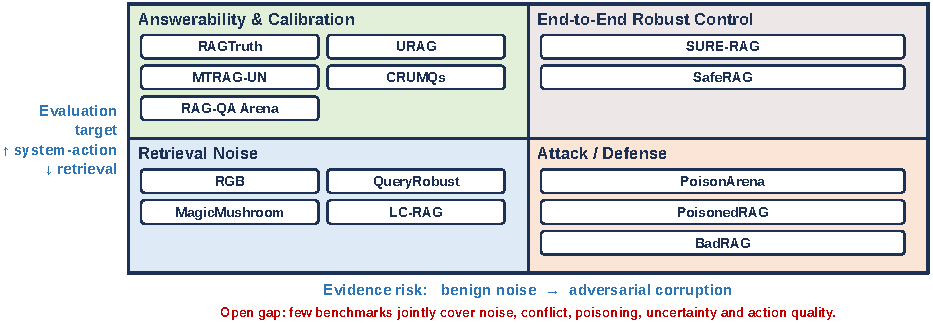
\includegraphics[width=\textwidth]{figures/generated/fig_benchmark_landscape.pdf}%
\caption{Conceptual benchmark landscape. Placement is illustrative rather than
data-derived; the figure organises differences in evidence risk and evaluation
level, not empirical distance or benchmark quality. The two axes are
coordinates C1 and C4, and the open gap is the reason a single ``robustness''
number rarely transfers between quadrants.}
\label{fig:benchmark-landscape}
\end{figure*}

\begin{table*}[t]
\centering
\scriptsize
\renewcommand{\arraystretch}{0.95}
\begin{tabularx}{\linewidth}{>{\raggedright\arraybackslash}p{0.12\linewidth}>{\raggedright\arraybackslash}p{0.13\linewidth}>{\raggedright\arraybackslash}p{0.17\linewidth}>{\raggedright\arraybackslash}p{0.18\linewidth}>{\raggedright\arraybackslash}p{0.14\linewidth}X}
\toprule
\textbf{Benchmark} & \textbf{Risk focus} & \textbf{Task / data} & \textbf{Perturbation or threat} & \textbf{Metrics} & \textbf{Boundary} \\
\midrule
RGB \citep{rgb2023} & noise, rejection, integration, counterfactuality & English/Chinese QA & noisy passages, false evidence, negative evidence & accuracy, ability-specific scores & Broad diagnostic benchmark but not adaptive attack-oriented. \\
RAGTruth \citep{ragTruth2024} & hallucination / faithfulness & QA, data-to-text, summarization & naturally generated unsupported spans & word-level hallucination labels & Strong annotation granularity; less focused on retrieval-side threat models. \\
Sufficient Context \citep{sufficientContext2024} & answerability & QA with context sufficiency labels & insufficient retrieved evidence & selective generation / abstention & Captures answerability but not adversarial corruption. \\
MagicMushroom \citep{rrag027} & retrieval noise & configurable RAG stress tests & distracting, low-quality, inconsequential, irrelevant noise & robustness under noise types & Fine-grained noise; limited conflict/security coverage. \\
URAG \citep{rrag001} & uncertainty & RAG as MCQA / conformal prediction & irrelevant/noisy retrieval and uncertainty sets & coverage, set size, calibration & Good for uncertainty; less direct for free-form generation. \\
QueryRobust \citep{queryRobustness2025} & query robustness & QA with query perturbations & wording variation at query--retrieval interface & retrieval and end-task degradation & Focuses on query perturbation, not corpus corruption. \\
PoisonArena \citep{rrag023} & adversarial poisoning & RAG attack competition setting & competing poisoning attacks & attack success, retrieval effects & Strong security focus; benign uncertainty is secondary. \\
SafeRAG \citep{rrag019} & RAG security & security benchmark for RAG & poisoning / malicious retrieval contexts & attack and defense metrics & Security-oriented; not a full evidence reliability suite. \\
MTRAG-UN \citep{rrag141} & multi-turn unanswerability & multi-turn RAG conversations & unanswerable, underspecified, non-standalone questions & abstention / clarification quality & Covers interaction; less focused on adversarial evidence. \\
CRUMQs \citep{rrag193} & unanswerable multi-hop RAG & realistic multi-hop queries & unanswerable and uncheatable questions & answerability and robustness & Useful for abstention; not a broad attack/noise benchmark. \\
\bottomrule
\end{tabularx}
\caption{Benchmark-level comparison for robust RAG evaluation. The table makes explicit what each benchmark perturbs, what it measures, and which failure modes remain outside its scope.}
\label{tab:benchmark-comparison}
\end{table*}


\begin{table*}[t]
\centering
\scriptsize
\begin{tabularx}{\linewidth}{p{0.18\linewidth}p{0.22\linewidth}p{0.24\linewidth}X}
\toprule
\textbf{Benchmark component} & \textbf{Required annotation} & \textbf{Metric suite} & \textbf{Why it is needed} \\
\midrule
Evidence reliability & relevance, sufficiency, freshness, provenance, support span & retrieval recall, sufficient-context accuracy, support precision & Distinguishes merely related passages from answer-supporting evidence. \\
Distraction and conflict & distractor type, conflicting claim pair, source agreement & answer flip rate, conflict sensitivity, context-utilisation score & Reveals whether models ignore harmful context or silently pick a source. \\
Adversarial corruption & attacker access, insertion budget, trigger type, poisoned document ID & attack success, poisoned retrieval rate, stealth, defense bypass & Makes security results comparable across threat models. \\
Unanswerability and ambiguity & answerability label, ambiguity type, clarification target & selective risk, abstention precision/recall, clarification accuracy & Evaluates robust action selection, not just answer generation. \\
Cost and system action & number of retrievals, verifier calls, latency, final action trace & cost-adjusted accuracy, action utility, coverage--risk curve & Prevents methods from hiding robustness gains behind unbounded computation. \\
\bottomrule
\end{tabularx}
\caption{A proposed benchmark blueprint for robust RAG under unreliable evidence. This is a research agenda rather than a validated leaderboard; existing benchmarks cover parts of the schema.}
\label{tab:benchmark-blueprint}
\end{table*}

\begin{table*}[t]
\centering
\scriptsize
\renewcommand{\arraystretch}{0.88}
\begin{tabularx}{\linewidth}{>{\raggedright\arraybackslash}p{0.16\linewidth}>{\raggedright\arraybackslash}p{0.20\linewidth}>{\raggedright\arraybackslash}p{0.20\linewidth}>{\raggedright\arraybackslash}p{0.18\linewidth}X}
\toprule
\textbf{Pilot item type} & \textbf{Evidence state label} & \textbf{Correct action trace} & \textbf{Answer metric alone would say} & \textbf{Action-aware diagnosis} \\
\midrule
Benign hard negative & Gold evidence present; hard negative ranked above it & retrieve $\rightarrow$ rerank/filter $\rightarrow$ answer with support & Correct/incorrect answer & Separates retriever ranking error from generator distraction. \\
Insufficient context & Retrieved context related but lacks answer-bearing span & retrieve $\rightarrow$ detect insufficiency $\rightarrow$ re-retrieve or abstain & Wrong answer or refusal & Rewards abstention/retrieval control rather than forced guessing. \\
Retrieved conflict & Two sources disagree with different dates/provenance & retrieve $\rightarrow$ compare sources $\rightarrow$ expose conflict or prefer fresher source & One answer may match gold & Checks whether the system hides unresolved conflict. \\
Poisoned evidence & Malicious document retrieved with plausible support & retrieve $\rightarrow$ detect/demote/quarantine $\rightarrow$ answer or abstain & Attack success/failure & Distinguishes poisoned retrieval, defense detection, and final answer steering. \\
\bottomrule
\end{tabularx}
\caption{Illustrative action-trace pilot for the benchmark blueprint. This is a worked annotation example, not a released leaderboard or empirical system ranking.}
\label{tab:action-trace-pilot}
\end{table*}


\begin{table}[t]
\centering
\small
\begin{tabular}{lrrr}
\toprule
\textbf{Toy policy} & \textbf{Ans.} & \textbf{Act.} & \textbf{Joint} \\
\midrule
Answer-only & 0.25 & 0.25 & 0.25 \\
Abstain-on-missing & 0.67 & 0.50 & 0.50 \\
Evidence-action oracle & 1.00 & 1.00 & 1.00 \\
\bottomrule
\end{tabular}
\caption{Action-trace pilot over 12 synthetic diagnostic items. Answer accuracy, action accuracy, and joint answer-action accuracy diagnose different behavior.}
\label{tab:action-trace-pilot-results}
\end{table}


\begin{table*}[t]
\centering
\scriptsize
\renewcommand{\arraystretch}{0.92}
\begin{tabularx}{\linewidth}{>{\raggedright\arraybackslash}p{0.17\linewidth}>{\raggedright\arraybackslash}p{0.27\linewidth}>{\raggedright\arraybackslash}p{0.25\linewidth}X}
\toprule
\textbf{Axis} & \textbf{Typical variation across papers} & \textbf{Why conclusions fail to transfer} & \textbf{Minimum reporting requirement} \\
\midrule
Retriever/generator setting & BM25 vs dense vs hybrid retrieval; small vs frontier generators; frozen vs fine-tuned models & A defense may work by compensating for one retriever or one model scale rather than solving the failure mode. & Retriever, index, top-$k$, reranker, generator, prompt, decoding, and context length. \\
Attack budget and access & Poisoned-document count, corpus write access, query control, retriever visibility, generator access & Attack success rates are incomparable when one attacker edits a corpus and another only controls the query. & Capability matrix, insertion budget, target set, stealth objective, and whether malicious evidence is retrieved. \\
Metric target & EM/F1, faithfulness, citation support, attack success, calibration error, selective risk, cost & Improving answer accuracy can worsen citation faithfulness; improving abstention can reduce coverage; reducing attacks can lower utility. & Report utility, evidence support, risk, calibration, cost, and security as a Pareto surface. \\
Statistical and reproducibility evidence & Single seed/model vs multiple seeds/models; code/data availability varies & Small prompt or model changes can reverse robustness rankings, especially for LLM-as-judge or attack benchmarks. & Seeds, confidence intervals or bootstrap tests where feasible, released prompts, data splits, and code or exact API settings. \\
Long-context baseline & RAG-only comparisons vs long-context LLMs with the same documents & A robustness gain may reflect retrieval compression rather than evidence reliability control. & Include a long-context or full-context baseline when context length permits, and report latency/cost. \\
Attribution vs answer accuracy & Some tasks score only final answer; others require evidence-supported citations & A model can answer correctly for the wrong reason, cite irrelevant evidence, or ignore retrieved support. & Claim-level support labels, citation precision/recall, and answer correctness reported separately. \\
\bottomrule
\end{tabularx}
\caption{Evaluation-assumption matrix for robust RAG. The table summarises why benchmark results often cannot be compared without aligning system setup, threat model, metric target, reproducibility evidence, and long-context baselines.}
\label{tab:evaluation-assumption-matrix}
\end{table*}



Evaluation must reflect the full hierarchy. Standard exact match, F1, and retrieval recall remain useful but insufficient. A RAG system can retrieve relevant evidence and still answer from a distractor; it can answer correctly but be overconfident; it can refuse correctly but fail to explain what evidence is missing; it can pass benign noise tests but fail under poisoned corpora. Robust evaluation must therefore measure both failure resistance and action quality.

We group robust RAG evaluation into six families:
\begin{enumerate}[leftmargin=*]
    \item \textbf{Noise robustness}: performance as irrelevant or misleading passages are injected, removed, reordered, or ranked higher.
    \item \textbf{Distraction sensitivity}: whether answer or confidence changes when distractors are added while gold evidence remains available.
    \item \textbf{Conflict sensitivity}: whether the system detects and resolves parametric--retrieved or retrieved--retrieved contradictions.
    \item \textbf{Adversarial robustness}: attack success rate, poisoned retrieval rate, trigger robustness, defense bypass rate, and recovery after filtering.
    \item \textbf{Uncertainty and selective prediction}: selective risk, abstention precision/recall, expected calibration error, and clarification quality.
    \item \textbf{End-to-end action quality}: whether the system chooses the right policy among answer, retrieve, re-retrieve, filter, abstain, or ask.
\end{enumerate}
Benchmarking work such as RGB, RAGTruth, robustness-at-query-level analyses, poisoning benchmarks, and uncertainty benchmarks provides pieces of this landscape \citep{rgb2023,ragTruth2024,queryRobustness2025}. RGB is useful because it separates RAG abilities rather than reporting one score \citep{rgb2023}. RAGTruth contributes fine-grained hallucination annotations that support detection and attribution \citep{ragTruth2024}. Query-level robustness work shows that the query--retrieval interface is itself fragile \citep{queryRobustness2025}. PoisonArena-style benchmarks and LIAR-style attack evaluations stress adversarial settings rather than benign retrieval noise \citep{rrag023,rrag035}. URAG and uncertainty benchmarks evaluate whether systems know when their answers are reliable \citep{rrag001,rrag093}.

The main gap is joint evaluation. Most benchmarks isolate one failure: noise, conflict, poisoning, or unanswerability. In plausible high-risk document-grounded settings, these failures can interact: a query may be ambiguous, retrieval may surface partially relevant evidence, a document may be stale, and one source may be malicious or misleading. A future benchmark should therefore cross product failure types: benign hard negatives, conflicting evidence, poisoned passages, query perturbations, and insufficient context. It should also report action metrics: when the system retrieves, when it filters, when it verifies, when it abstains, and whether these actions improve risk--cost tradeoffs.

Table~\ref{tab:benchmark-blueprint} turns this observation into a proposed benchmark schema. We treat it as a research agenda, not as a validated benchmark contribution: no leaderboard or empirical re-ranking is claimed. The key design choice is to annotate not only answers but also evidence states and action traces. Without evidence annotations, a model can receive credit for an answer supported by parametric memory rather than retrieved evidence. Without action traces, a system that repeatedly retrieves, verifies, and self-consistently samples can look more robust while hiding its cost. Without attacker capability fields, security benchmark results become incomparable.

To make the proposal concrete, we include a 12-item synthetic action-trace pilot with three toy policies (Table~\ref{tab:action-trace-pilot-results}). The pilot is not a benchmark release, but it demonstrates the diagnostic difference: an answer-only policy can receive some answer credit while failing action quality, whereas action-aware scoring distinguishes answer correctness, control behavior, and their joint success.

Table~\ref{tab:evaluation-assumption-matrix} makes the comparison problem more explicit. Many reported gains depend on retriever choice, generator scale, context length, poisoning budget, and metric target. A method can improve EM while worsening citation support; a defense can reduce attack success while reducing answer utility; a retrieval policy can increase accuracy while hiding cost. We therefore treat robust-RAG evaluation as a multi-axis reporting problem rather than a leaderboard scalar.

\paragraph{A concrete benchmark protocol.}
An executable robust-RAG benchmark should instantiate the following template. Each item contains a user query, a gold answer or abstention/clarification target, a corpus snapshot with document IDs, a retrieved-context candidate set, and labels for supporting, distracting, conflicting, stale, poisoned, and insufficient evidence. The benchmark should define four splits: benign retrieval noise, knowledge conflict, adversarial corruption, and answerability uncertainty. For each split, systems must output both an answer and an action trace: whether they retrieved, filtered, verified, re-retrieved, abstained, or asked for clarification. The metric suite should report answer utility, evidence support precision, attack success or defense bypass where applicable, calibration/coverage, and cost-adjusted action utility. This protocol makes it possible to compare systems that answer directly against systems that spend additional computation on verification or abstention.

\subsection{Metric Design}

Robust RAG metrics should be diagnostic. For retrieval, recall and nDCG should be complemented by negative-utility metrics that penalise distracting evidence \citep{rrag058}. For generation, exact match should be complemented by faithfulness, citation support, and claim-level entailment. For attacks, attack success rate should be paired with stealth, retrieval rate, injected-document budget, and transferability. For calibration, expected calibration error should be paired with selective risk and coverage. For control, the unit of evaluation should be an action trace: retrieve, filter, verify, answer, abstain, or ask clarification. This makes it possible to distinguish a lucky correct answer from a robust decision process.

\subsection{Benchmark Construction Principles}

We identify four principles for future benchmark construction. First, benchmarks should include both benign and adversarial evidence unreliability. Second, they should provide source-level annotations: which passage supports which claim, which passage is distracting, which passage is poisoned, and which source conflicts with which. Third, they should include unanswerable and underspecified questions so that abstention and clarification can be evaluated. Fourth, they should report cost and latency, because robust RAG methods often trade reliability for additional computation. Benchmarks that omit these dimensions risk rewarding systems that answer more often rather than systems that answer more responsibly.
